\label{subseq:final-results}


Figures \ref{fig:mumps-final-comparison-1} and \ref{fig:mumps-final-comparison-2} show comparisons of \acrshort{mumps} parallel performance before and after application of the optimal \acrshort{mumps} settings, found in subsections \ref{subseq:fill-in-reordering}, \ref{subseq:mm-mumps-process-pinning}, \ref{subseq:blas-comparison}, and \ref{subseq:mpi-openmp}, to \acrshort{grs} matrix set. Results labeled as \textit{default} were obtained using the fill reducing reordering algorithm provided by ParMetis library because it had been used by \acrshort{athlet} users before the current study.\\


%\figpointer{\ref{fig:mumps-final-comparison-1}}
\begin{figure}[h!]
\centering
	\begin{tabular}{cc}
		\subfloat[small system: cube-5\label{fig:mumps-final-comparison-cube-5}]{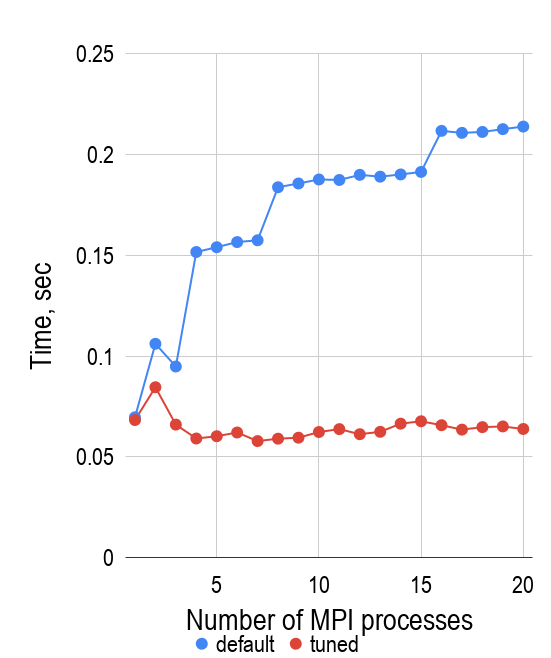
\includegraphics[width=0.41\textwidth]{figures/chapter-2/final-comparison/cube-5.png}} &
		\subfloat[small system: pwr-3d\label{fig:mumps-final-comparison-pwr-3d}]{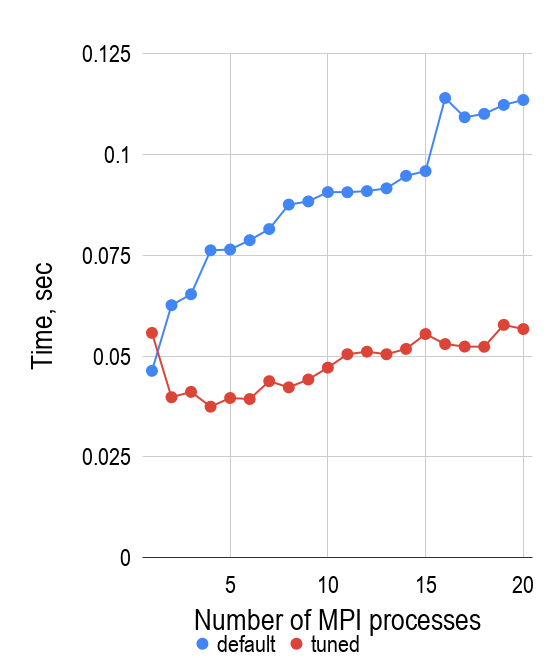
\includegraphics[width=0.41\textwidth]{figures/chapter-2/final-comparison/pwr-3d.png}} \\
		\subfloat[medium system: cube-64]{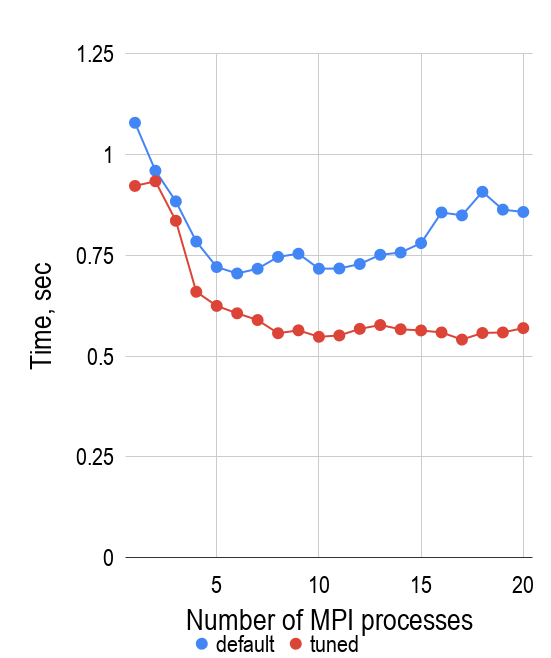
\includegraphics[width=0.41\textwidth]{figures/chapter-2/final-comparison/cube-64.png}} & 			        \subfloat[medium system: k3-2]{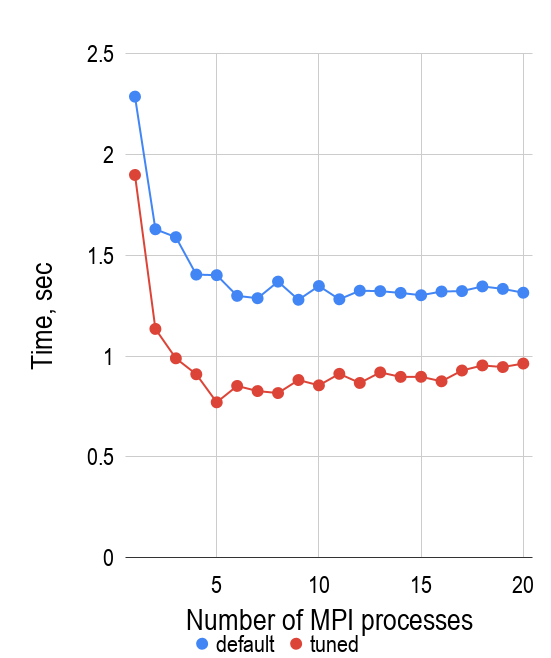
\includegraphics[width=0.41\textwidth]{figures/chapter-2/final-comparison/k3-2.png}} \\
	\end{tabular}
	\caption{Comparisons of parallel factorizations of small- and middle-sized \acrshort{grs} matrices between applications of the default and optimal MUMPS configurations}
	\label{fig:mumps-final-comparison-1}
\end{figure}



%\figpointer{\ref{fig:mumps-final-comparison-2}}
\begin{figure}
\centering
	\begin{tabular}{cc}
		\subfloat[large system: cube-645\label{fig:mumps-final-comparison-cube-645}]{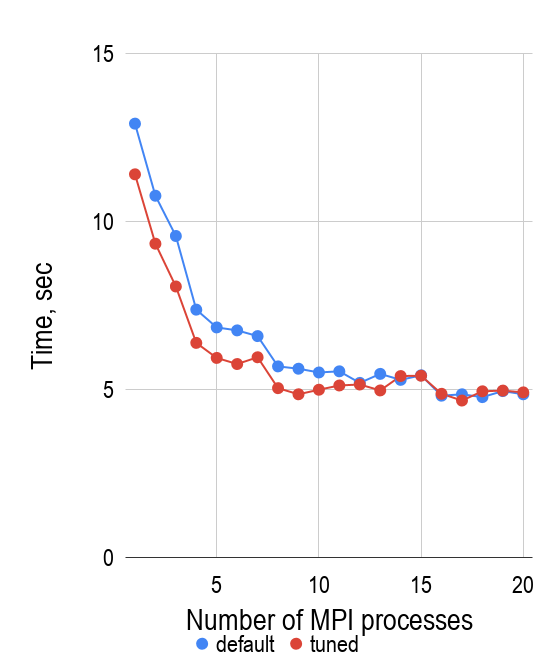
\includegraphics[width=0.43\textwidth]{figures/chapter-2/final-comparison/cube-645.png}} & 			        \subfloat[large system: k3-18\label{fig:mumps-final-comparison-k3-18}]{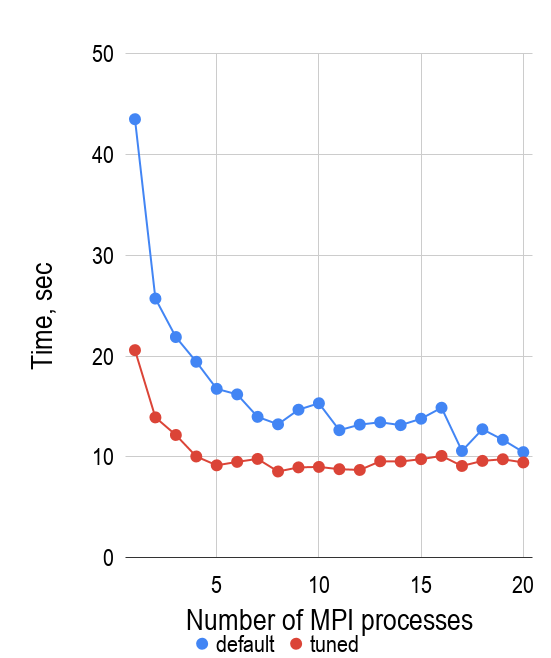
\includegraphics[width=0.43\textwidth]{figures/chapter-2/final-comparison/k3-18.png}} \\
	\end{tabular}
	\caption{Comparisons of parallel factorizations of large-sized \acrshort{grs} matrices between applications of the default and optimal MUMPS configurations}
	\label{fig:mumps-final-comparison-2}
\end{figure}

\newpage



On average, factorization time is reduced by \textbf{51.4\%} for small-sized linear systems, \textit{cube-5} and \textit{pwr-3d}. As it was expected, the most significant performance gain mainly comes from a correct choice of a fill reducing reordering algorithm. Moreover, application of PT-Scotch for these systems of equations results in a drastic change of strong scaling behavior, see figures \ref{fig:mumps-final-comparison-cube-5} and  \ref{fig:mumps-final-comparison-pwr-3d}, which allows to reduce execution time by approximately \textbf{17\%} in contrast to the sequential execution of \acrshort{mumps} running with the default parameters.\\


% medium sized systems
Execution time spent on factorization of medium-sized systems, such as \textit{cube-64} and \textit{k3-2}, drops in \textbf{1.4} times on an average. We have noticed that strong scaling of \textit{cube-64} test-case considerably improves. Additionally, application of PT-Scotch to \textit{cube-64} matrix results in shifting of the optimal \acrshort{mpi} process count, the saturation point, from 5 to 10 and, as a result, it improves efficiency of the solver. Applied settings reduce execution time around the corresponding saturation points by almost \textbf{31\%} on average for these type of \acrshort{grs} matrices.\\


% larged sized sized system
%Only optimal processes pinning and application of OpenBLAS library result in parallel performance gain of large-sized systems because of usage of the same fill reducing reordering algorithm, ParMetis.

Improvements in parallel factorization of large-sized \acrshort{grs} systems comes only from optimal processes pinning and application of OpenBLAS library because of the usage of the same optimal fill reducing reordering algorithm, ParMetis. On average, performance increased almost by \textbf{20\%} in case of \textit{k3-18} test-case and only by \textbf{1.3\%} for \textit{cube-645} one. This difference in results can be explained by the fact that the assembly tree of \textit{cube-645} test-case lacks type 2 nodes. However, the saturation points of both test-cases are shifted towards lower values of the \acrshort{mpi} process count which results in a considerably improvement of hardware utilization. For example, a detailed study of \textit{k3-18} performance graph, figure \ref{fig:mumps-final-comparison-k3-18}, shows the optimal \acrshort{mpi} process count value decreases from 17 to 8 and, at the same time, execution time drops by almost \textbf{19\%}. These two effects result in almost \textbf{13\%} jump of parallel efficiency. The same trend can be observed for \textit{cube-645} test-case as well.\\


By and large, in this subsection we have shown the application of the optimal parameters to \acrshort{mumps} leads to total accumulative improvements in factorization time and hardware utilization.\\



%average
% shit of saturation point
% usage of less amount of processing units helps to improve efficiency of the system
% example of k-18, k3-2
% recomendations for small, medium and big GRS systems
